\chapter{Introduction}
\label{c:intro}

\newcommand{\FourQueens}[2] {
  \begin{tikzpicture}[scale=0.6, every node/.style={black,scale=0.9}]
    \newcommand*{\xMin}{0}%
    \newcommand*{\xMax}{3}%
    \newcommand*{\yMin}{0}%
    \newcommand*{\yMax}{3}%
    \foreach \i / \label in {0/a,1/b,2/c,3/d} {
        \draw [] node at (\i+.5,\yMin-.3) {$\label$};
    }
    \foreach \i / \label in {0/1,1/2,2/3,3/4} {
        \draw [] node at (\xMin-.3,\i+.5) {$\label$};
    }

    \foreach \y in {0,2}{
        \foreach \x in {0,2}{
            \fill[black!8] (\x,\y) rectangle (1+\x,1+\y) rectangle (2+\x,2+\y);}}
    \draw [step=1.0] (0,0) grid (4,4);
    \foreach \x/\y/\m in {#2}
        \draw [] node at (\x,\y) {\m};
    \node[draw,circle,inner sep=1mm] at (-1.4,3.5) {#1};
  \end{tikzpicture}
}

\newcommand{\MCSDomains}[2] {
  \begin{tikzpicture}[scale=0.6, every node/.style={black,scale=0.9}]
    \newcommand*{\xMin}{0}%
    \newcommand*{\xMax}{5}%
    \newcommand*{\yMin}{0}%
    \newcommand*{\yMax}{4}%
    \foreach \i / \label in {0/a,1/b,2/c,3/d,4/e,5/f} {
        \draw [] node at (\i+.5,\yMax+1.4) {$\label$};
    }
    \foreach \i / \label in {4/1,3/2,2/3,1/4,0/5} {
        \draw [] node at (\xMin-.3,\i+.5) {$\label$};
    }

    \draw [step=1.0] (0,0) grid (6,5);
    \foreach \x/\y/\m in {#2}
        \draw [] node at (\x,\y) {\m};
    \node[draw,circle,inner sep=1mm] at (-1.4,3.5) {#1};
  \end{tikzpicture}
}

Graphs --- collections of items (vertices), some pairs of which
are related --- can be used to model
systems from a huge variety of domains.  A molecule can be viewed as a collection
of vertices (the atoms) joined together by bonds
\citep{sussenguth1965graph}; 
an image may be summarised using a vertex for each coloured region
with adjacent vertices joined \citep{DBLP:conf/icip/OlatunbosunDE96}.
We may wish to determine whether all or a large
part of a given object --- such as a molecule or image --- is contained
in another given object.  This dissertation presents new algorithms
for such problems.

The first problem we consider is the \emph{maximum common induced subgraph}
family of problems: we seek to find a large subgraph that is
contained in each of two given graphs.
Depending on the flavour of the problem, these
graphs may be directed or undirected and may or may not have labels.
All of these variants of the can be handled by the \McSplit\ family of algorithms.
These algorithms use a simple, fast and space-efficient data structure to keep
track of the set of vertices in the second graph to which a given vertex
in the first graph may be mapped.

The second problem we consider is \emph{induced subgraph isomorphism}: to determine
whether a given graph (the ``target graph'') contains another given graph (the ``pattern graph'')
as an induced subgraph.  We again use a variant of the \McSplit\ algorithm ---
\McSplit-SI --- to solve the problem; this version of the algorithm has a specialised
version of \McSplit's data structure that allows very fast processing of sparse graphs.

For the final problem considered in this dissertation, we turn from subgraphs
to supergraphs.  We study the problem of finding, for a given family of graphs,
an \textit{induced universal graph} --- that is, a graph that contains every
member of the family as an induced subgraph --- with as few vertices as
possible.  This problem generalises the \textit{minimum common supergraph}
problem to an arbitrary number of input graphs.  Although much progress has
been made on asymptotic results on the size of induced universal graphs, almost no
work has been done on developing algorithms to solve the problem exactly.  This
dissertation presents an algorithm for finding minimal induced universal graphs
using \McSplit-SI as a subroutine, and presents new terms of integer sequences
generated using the program.  Further, we present a hill-climbing method for
finding small (although possibly not optimal) induced universal graphs.

\section{Preliminaries}

A graph $G$ is a pair $(V, E)$ whose \emph{vertex set} $V = V(G)$
is an arbitrary finite set and whose \emph{edge set} $E = E(G)$
comprises two-elements subset of $V$. The elements of each edge
$e \in E$ are called its \emph{endpoints}, and two vertices that
are the endpoints of some edge are said to be \emph{adjacent}.

For example, \Cref{fig:g1} shows the graph $G_1 = (V,E)$, where
\[
V = \{1, 2, 3, 4, 5, 6\},
E = \{\{1,2\}, \{1,3\}, \{2,3\}, \{3,4\}, \{4,5\}, \{4,6\}, \{5,6\}\}
.
\]

\begin{figure}[htb]
    \centering
    \subfigure[][$G_1$] {
        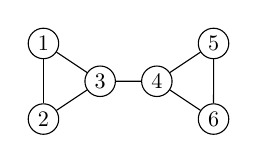
\begin{tikzpicture}[scale=0.6, every node/.style={scale=0.8,inner sep=.7mm}]
          \node [draw,circle] (1) at (0,1.6) {1};
          \node [draw,circle] (2) at (0,0) {2};
          \node [draw,circle] (3) at (1.2,.8) {3};
          \node [draw,circle] (4) at (2.4,.8) {4};
          \node [draw,circle] (5) at (3.6,1.6) {5};
          \node [draw,circle] (6) at (3.6,0) {6};
          \draw (1) -- (2);
          \draw (1) -- (3);
          \draw (2) -- (3);
          \draw (3) -- (4);
          \draw (4) -- (5);
          \draw (4) -- (6);
          \draw (5) -- (6);
        \end{tikzpicture}
        \label{fig:g1}
    }
    \quad\subfigure[][$G_2$] {
        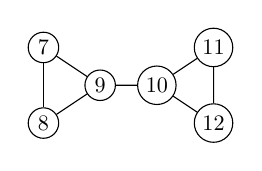
\begin{tikzpicture}[scale=0.6, every node/.style={scale=0.8,inner sep=.7mm}]
          \node [draw,circle] (1) at (0,1.6) {7};
          \node [draw,circle] (2) at (0,0) {8};
          \node [draw,circle] (3) at (1.2,.8) {9};
          \node [draw,circle] (4) at (2.4,.8) {10};
          \node [draw,circle] (5) at (3.6,1.6) {11};
          \node [draw,circle] (6) at (3.6,0) {12};
          \draw (1) -- (2);
          \draw (1) -- (3);
          \draw (2) -- (3);
          \draw (3) -- (4);
          \draw (4) -- (5);
          \draw (4) -- (6);
          \draw (5) -- (6);
        \end{tikzpicture}
        \label{fig:g2}
    }
    \quad\subfigure[][$G_3$] {
        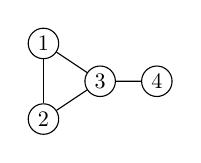
\begin{tikzpicture}[scale=0.6, every node/.style={scale=0.8,inner sep=.7mm}]
          \node [draw,circle] (1) at (0,1.6) {1};
          \node [draw,circle] (2) at (0,0) {2};
          \node [draw,circle] (3) at (1.2,.8) {3};
          \node [draw,circle] (4) at (2.4,.8) {4};
          \draw (1) -- (2);
          \draw (1) -- (3);
          \draw (2) -- (3);
          \draw (3) -- (4);
        \end{tikzpicture}
        \label{fig:g3}
    }
%    \quad\subfigure[][$G_4$] {
%        \begin{tikzpicture}[scale=0.6, every node/.style={scale=0.8,inner sep=.7mm}]
%          \node [draw,circle] (1) at (0,1.6) {1};
%          \node [draw,circle] (2) at (0,0) {2};
%          \node [draw,circle] (3) at (1.2,.8) {3};
%          \node [draw,circle] (4) at (2.4,1.6) {4};
%          \node [draw,circle] (5) at (2.4,0) {5};
%          \draw (1) -- (2);
%          \draw (1) -- (3);
%          \draw (2) -- (3);
%          \draw (3) -- (4);
%          \draw (3) -- (5);
%          \draw (4) -- (5);
%        \end{tikzpicture}
%        \label{fig:g4}
%    }
    \caption{Example graphs $G_1$ to $G_3$}
    \label{fig:intro-examples}
\end{figure}

A \emph{loop} is an edge from a vertex to itself. We assume throughout this
dissertation that graphs have no loops, except in clearly marked sections where
we discuss extensions of algorithms to graphs with loops.

The set of vertices adjacent to vertex $v \in V(G)$
is called the \emph{neighbourhood} of $v$, denoted $\N_G(v)$. We denote
by $\invN_G(v)$ the \emph{inverse neighbourhood} of $v$: the set
of the vertices other than $v$ itself that are not adjacent to $v$.
We omit the subscript $G$ where there is no ambiguity.
In \Cref{fig:g1}, for example, we have $\N(3) = \{1,2,4\}$ and
$\invN(3) = \{5,6\}$.

We say that graphs $G$ and $H$ are \emph{isomorphic} if we can relabel
the vertices of $G$ to produce graph $H$. For example, graphs $G_1$
and $G_2$ in \Cref{fig:intro-examples} are isomorphic.
Formally, an isomorphism between graphs $G$ and $H$ is a bijection $f$
from $V(G)$ to $V(H)$, such that $E(H) = \{\{f(u), f(v)\} \mid \{u, v\} \in E(G)\}$.
If such an $f$ exists, we say that $G$ and $H$ are isomorphic.

An \emph{induced subgraph} of $G = (V, E)$ has a subset $W \subseteq V$ as its
vertex set, and $\{\{u, v\} \in E \mid \{u, v\} \in W\}$ as its edge set; that
is, the subgraph includes all edges of $G$ whose endpoints both appear in
$W$.  We say that this subgraph is \emph{induced by} $W$.
Graph $G_3$ of \Cref{fig:intro-examples} is thus the subgraph
of $G_1$ induced by the set $\{1,2,3,4\}$.
A \emph{subgraph} (without the ``induced'' qualifier) is an induced subgraph
with zero or more of the edges deleted.

A \emph{common induced subgraph} of graphs $G$ and $H$ is an induced subgraph
of $G$ which is isomorphic to an induced subgraph of $H$. In
\Cref{fig:cis-example}, a common induced subgraph of the two graphs (which is
induced by $\{1,2,3,4\}$) is highlighted on the first graph, and its isomorphic
subgraph is highlighted on the second graph.  It is often convenient to summarise
a common induced subgraph and its associated isomorphism $f$ by the \emph{mapping}
$\{(v,f(v)) \mid v \in W\}$, where $W \subseteq V$ is the set of vertices that
induces the common subgraph.  In our example, $M = \{(1,6), (2,7), (3,8), (4,9)\}$.

\begin{figure}[h!]
\centering
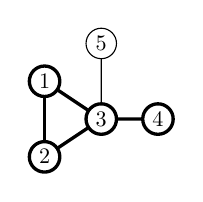
\begin{tikzpicture}[scale=0.6, every node/.style={scale=0.8,inner sep=.7mm}]
  \node [very thick,draw,circle] (1) at (0,1.6) {1};
  \node [very thick,draw,circle] (2) at (0,0) {2};
  \node [very thick,draw,circle] (3) at (1.2,.8) {3};
  \node [very thick,draw,circle] (4) at (2.4,.8) {4};
  \node [draw,circle] (5) at (1.2,2.4) {5};
  \draw [very thick] (1) -- (2);
  \draw [very thick] (1) -- (3);
  \draw [very thick] (2) -- (3);
  \draw [very thick] (3) -- (4);
  \draw (3) -- (5);
\end{tikzpicture}
\qquad
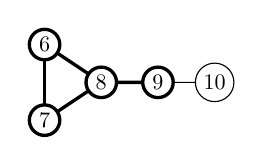
\begin{tikzpicture}[scale=0.6, every node/.style={scale=0.8,inner sep=.7mm}]
  \node [very thick,draw,circle] (1) at (0,1.6) {6};
  \node [very thick,draw,circle] (2) at (0,0) {7};
  \node [very thick,draw,circle] (3) at (1.2,.8) {8};
  \node [very thick,draw,circle] (4) at (2.4,.8) {9};
  \node [draw,circle] (5) at (3.6,.8) {10};
  \draw [very thick] (1) -- (2);
  \draw [very thick] (1) -- (3);
  \draw [very thick] (2) -- (3);
  \draw [very thick] (3) -- (4);
  \draw (4) -- (5);
\end{tikzpicture}
\caption{A pair of graphs with a maximum common induced subgraph highlighted}
\label{fig:cis-example}
\end{figure}

A \emph{maximum common induced subgraph (MCIS)} of $G$ and $H$ is a common
induced subgraph of $G$ and $H$ whose vertex set is as large as possible; the
common induced subgraph in \Cref{fig:cis-example} is an example of an MCIS.

A \emph{labelled graph} (or \emph{network}) is a triple $(G, f_v, f_e)$
where $G$ is a graph,
the \emph{vertex label function} $f_v$ is a function with domain $V(G)$,
and the \emph{edge label function} $f_e$ is a function with domain $E(G)$.
The maximum common induced subgraph problem has a natural extension to labelled graphs
where we require the isomorphism to preserve labels on vertices and edges.

A \emph{directed graph} is a pair $(V,A)$, where $V$ is the vertex set and $A$,
a set of ordered pairs of elements of $V$, is the arc set.  The definitions of
\emph{induced subgraph}, \emph{isomorphism} and \emph{maximum common induced
subgraph} for directed graphs are analogous to their counterparts for graphs.
\label{fig:directed-cis-example} shows two directed graphs with a common
induced subgraph highlighted.

\begin{figure}[h!]
\centering
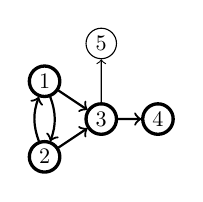
\begin{tikzpicture}[scale=0.6, every node/.style={scale=0.8,inner sep=.7mm}]
  \node [very thick,draw,circle] (1) at (0,1.6) {1};
  \node [very thick,draw,circle] (2) at (0,0) {2};
  \node [very thick,draw,circle] (3) at (1.2,.8) {3};
  \node [very thick,draw,circle] (4) at (2.4,.8) {4};
  \node [draw,circle] (5) at (1.2,2.4) {5};
  \draw [->,thick,bend left=20] (1) edge (2);
  \draw [->,thick,bend left=20] (2) edge (1);
  \draw [->,thick] (1) edge (3);
  \draw [->,thick] (2) edge (3);
  \draw [->,thick] (3) edge (4);
  \draw [->] (3) edge (5);
\end{tikzpicture}
\qquad
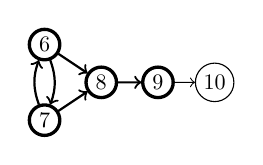
\begin{tikzpicture}[scale=0.6, every node/.style={scale=0.8,inner sep=.7mm}]
  \node [very thick,draw,circle] (1) at (0,1.6) {6};
  \node [very thick,draw,circle] (2) at (0,0) {7};
  \node [very thick,draw,circle] (3) at (1.2,.8) {8};
  \node [very thick,draw,circle] (4) at (2.4,.8) {9};
  \node [draw,circle] (5) at (3.6,.8) {10};
  \draw [->,thick,bend left=20] (1) edge (2);
  \draw [->,thick,bend left=20] (2) edge (1);
  \draw [->,thick] (1) edge (3);
  \draw [->,thick] (2) edge (3);
  \draw [->,thick] (3) edge (4);
  \draw [->] (4) edge (5);
\end{tikzpicture}
\caption{A pair of directed graphs with a maximum common induced subgraph highlighted}
\label{fig:directed-cis-example}
\end{figure}

For arc $(u,v)$, we say that $u$ is the source vertex and $v$ is target vertex; both
$u$ and $v$ are called endpoints.

\section{Problems covered by this dissertation}

This dissertation presents algorithms for the following three problems.

\begin{itemize}
    \item \textbf{Maximum common induced subgraph.} Find
a maximum common induced subgraph of two given graphs.
    \item \textbf{Induced subgraph isomorphism.} Given graphs $G$ and $H$,
determine whether $G$ is isomorphic to an induced subgraph of $H$;
if so, return the isomorphism.
    \item \textbf{Minimum induced universal graph.} Given a family of graphs $\calF$,
find a graph with as few vertices as possible that contains each member of $\calF$
as an induced subgraph.
\end{itemize}

Each of the three problems can be seen to be NP-hard by a simple reduction from \textsc{Clique}.
Given graph $G$ and natural number $k$, we can determine whether $G$ contains a clique
of size $k$ by solving either of the first two problems with the complete graph $K_k$ as
the first graph and $G$ as the second, or by solving the third problem with the family
$\{K_k, G\}$ as input.

\section{Related Problems}

The \emph{graph isomorphism} problem is a special case of the induced subgraph
isomorphism problem in which the two input graphs have the same number of
vertices.  Most state of the art algorithms for graph isomorphism, such as
Nauty and Traces, solve the problem by computing a canonical representation of
each graph and comparing these representations \citep{McKay201494}.  The
canonical representations may then be re-used for comparisons with other
graphs.  Considering only pairwise comparisons of graphs, a 2001 study found
that the induced subgraph isomorphism solver VF2 outperformed Nauty on several
classes of graph \citep{foggia2001performance}.  While we do not consider graph
isomorphism further in this dissertation, it would be an interesting topic of
future work to test whether the current state of the art subgraph isomorphism
solvers outperform the best graph isomorphism solvers on some interesting
classes of graphs.

Maximum common induced subgraph and induced subgraph isomorphism each have a non-induced
counterpart. grib

We now consider the \emph{maximum common edge subgraph (MCES)} family of problems,
beginning with the simple case of undirected graphs. An edge subgraph of $(V, E)$
is any graph $(W, F)$ such that $W$ is a subset of $V$ and $F$ is a subset of $E$; the
subgraph may thus contain any subsets of the vertices and edges of the original
graph, as long as the subgraph’s vertex set contains all of the endpoints of
edges in its edge set. To give two examples, both graphs in Figure C are edge
subgraphs of the graph in Figure B. Every induced subgraph of a graph $G$ is also
an edge subgraph of $G$.

A common edge subgraph of graphs $G$ and $H$ is an edge subgraph of $G$ that is
isomorphic to an edge subgraph of $H$. A maximum common edge subgraph of two
graphs is a common edge subgraph with as many edges as possible.

MCIS generalises the induced subgraph isomorphism problem, which is the problem
of determining whether graph $G$ is isomorphic to an induced subgraph of graph $H$.
MCES generalises the non-induced subgraph isomorphism problem, which is to
determine whether $G$ is isomorphic to an edge subgraph of $H$. Both problems are
NP-complete; thus, all of the maximum common subgraph problems described so far
are NP-hard.

Both of the subgraph isomorphism problems generalise graph isomorphism, which
is to determine whether two graphs are isomorphic. ?? As we will discuss later,
our partitioning algorithms have similarities to graph isomorphism algorithms
such as Conauto.

The maximum clique problem is to find an induced subgraph of a graph $G$ with as
many vertices as possible, such that the subgraph has all possible edges; that
is ??. Maximum clique can be solved (although rather inefficiently in practice)
using an MCIS algorithm, by finding the MCIS of $G$ and a complete graph with the
same number of vertices as $G$.

\section{Existing Algorithms}

In this subsection, we outline the existing approaches for solving MCIS on
undirected graphs. Algorithms for other maximum common subgraph problems have
similarities to these approaches, and will be described in detail in later
chapters.

It is useful to introduce the concept of a mapping to denote a pair of common
subgraphs of input graphs $G$ and $H$ and the isomorphism between these subgraphs.
A mapping $M$ is a set of 2-tuples, where each tuple contains a vertex from the
first graph followed by a vertex from the second graph. The subgraph of $G$ is
induced by $\{u \mid (u, v) \in M\}$, and the subgraph of $H$ is induced by $\{v \mid (u, v)
\in M\}$. The isomorphism between these subgraphs is a function that maps each $u$
that appears as the first element of a 2-tuple to the second element of that
tuple.

The association graph of $G$ and $H$ is a graph with $\{(u,v) \mid u \in V(G) \wedge v \in
V(H)\}$ as its vertex set; it thus has $|V(G)||V(H)|$ vertices. Two vertices $(u,v)$
and $(u',v')$ in the association graph are adjacent if and only if all of the
following conditions are met.

\begin{itemize}
  \item $u \not= u'$
  \item $v \not= v'$
  \item $((u,u') \in E(G)) = ((v,v') \in E(H))$
\end{itemize}

A subset of the vertices of the association graph is a valid mapping if and
only if it is a clique in the association graph (?? proof?). Thus, we can find
an MCIS of G and H by running a maximum clique solver on the association graph
of G and H. Association graph encodings can be used to solve directed MCIS on
directed graphs and (with modifications) MCES.

\section{Backtracking Search}

TODO: describe search tree, CP, forward checking, levels of consistency.

\newsavebox{\FourQueensBoxA}
\newsavebox{\FourQueensBoxB}
\newsavebox{\FourQueensBoxC}
\newsavebox{\FourQueensBoxD}
\newsavebox{\FourQueensBoxE}
\newsavebox{\FourQueensBoxF}
\newsavebox{\FourQueensBoxG}
\newsavebox{\FourQueensBoxH}
\newsavebox{\FourQueensBoxI}
\sbox{\FourQueensBoxA}{\FourQueens{A}{0.5/0.5/,1.5/0.5/,2.5/0.5/,3.5/0.5/,0.5/1.5/,1.5/1.5/,2.5/1.5/,3.5/1.5/,0.5/2.5/,1.5/2.5/,2.5/2.5/,3.5/2.5/,0.5/3.5/,1.5/3.5/,2.5/3.5/,3.5/3.5/}}
\sbox{\FourQueensBoxB}{\FourQueens{B}{0.5/0.5/\symqueen,1.5/0.5/$\times$,2.5/0.5/$\times$,3.5/0.5/$\times$,0.5/1.5/$\times$,1.5/1.5/$\times$,2.5/1.5/,3.5/1.5/,0.5/2.5/$\times$,1.5/2.5/,2.5/2.5/$\times$,3.5/2.5/,0.5/3.5/$\times$,1.5/3.5/,2.5/3.5/,3.5/3.5/$\times$}}
\sbox{\FourQueensBoxC}{\FourQueens{C}{0.5/0.5/\symqueen,1.5/0.5/$\times$,2.5/0.5/$\times$,3.5/0.5/$\times$,0.5/1.5/$\times$,1.5/1.5/$\times$,2.5/1.5/\symqueen,3.5/1.5/$\times$,0.5/2.5/$\times$,1.5/2.5/$\times$,2.5/2.5/$\times$,3.5/2.5/$\times$,0.5/3.5/$\times$,1.5/3.5/,2.5/3.5/$\times$,3.5/3.5/$\times$}}
\sbox{\FourQueensBoxD}{\FourQueens{D}{0.5/0.5/\symqueen,1.5/0.5/$\times$,2.5/0.5/$\times$,3.5/0.5/$\times$,0.5/1.5/$\times$,1.5/1.5/$\times$,2.5/1.5/$\times$,3.5/1.5/\symqueen,0.5/2.5/$\times$,1.5/2.5/,2.5/2.5/$\times$,3.5/2.5/$\times$,0.5/3.5/$\times$,1.5/3.5/$\times$,2.5/3.5/,3.5/3.5/$\times$}}
\sbox{\FourQueensBoxE}{\FourQueens{E}{0.5/0.5/\symqueen,1.5/0.5/$\times$,2.5/0.5/$\times$,3.5/0.5/$\times$,0.5/1.5/$\times$,1.5/1.5/$\times$,2.5/1.5/$\times$,3.5/1.5/\symqueen,0.5/2.5/$\times$,1.5/2.5/$\times$,2.5/2.5/\symqueen,3.5/2.5/$\times$,0.5/3.5/$\times$,1.5/3.5/$\times$,2.5/3.5/$\times$,3.5/3.5/$\times$}}
\sbox{\FourQueensBoxF}{\FourQueens{F}{0.5/0.5/$\times$,1.5/0.5/\symqueen,2.5/0.5/$\times$,3.5/0.5/$\times$,0.5/1.5/$\times$,1.5/1.5/$\times$,2.5/1.5/$\times$,3.5/1.5/,0.5/2.5/,1.5/2.5/$\times$,2.5/2.5/,3.5/2.5/$\times$,0.5/3.5/,1.5/3.5/$\times$,2.5/3.5/,3.5/3.5/}}
\sbox{\FourQueensBoxG}{\FourQueens{G}{0.5/0.5/$\times$,1.5/0.5/\symqueen,2.5/0.5/$\times$,3.5/0.5/$\times$,0.5/1.5/$\times$,1.5/1.5/$\times$,2.5/1.5/$\times$,3.5/1.5/\symqueen,0.5/2.5/,1.5/2.5/$\times$,2.5/2.5/$\times$,3.5/2.5/$\times$,0.5/3.5/,1.5/3.5/$\times$,2.5/3.5/,3.5/3.5/$\times$}}
\sbox{\FourQueensBoxH}{\FourQueens{H}{0.5/0.5/$\times$,1.5/0.5/\symqueen,2.5/0.5/$\times$,3.5/0.5/$\times$,0.5/1.5/$\times$,1.5/1.5/$\times$,2.5/1.5/$\times$,3.5/1.5/\symqueen,0.5/2.5/\symqueen,1.5/2.5/$\times$,2.5/2.5/$\times$,3.5/2.5/$\times$,0.5/3.5/$\times$,1.5/3.5/$\times$,2.5/3.5/,3.5/3.5/$\times$}}
\sbox{\FourQueensBoxI}{\FourQueens{I}{0.5/0.5/$\times$,1.5/0.5/\symqueen,2.5/0.5/$\times$,3.5/0.5/$\times$,0.5/1.5/$\times$,1.5/1.5/$\times$,2.5/1.5/$\times$,3.5/1.5/\symqueen,0.5/2.5/\symqueen,1.5/2.5/$\times$,2.5/2.5/$\times$,3.5/2.5/$\times$,0.5/3.5/$\times$,1.5/3.5/$\times$,2.5/3.5/\symqueen,3.5/3.5/$\times$}}

\begin{figure}[h!]
\centering
\begin{forest}
[\usebox{\FourQueensBoxA}
  [\usebox{\FourQueensBoxB}
    [\usebox{\FourQueensBoxC}]
    [\usebox{\FourQueensBoxD} [\usebox{\FourQueensBoxE}]]
  ]
  [\usebox{\FourQueensBoxF}
    [\usebox{\FourQueensBoxG}
      [\usebox{\FourQueensBoxH}
        [\usebox{\FourQueensBoxI}]
      ]
    ]
  ]
]
\end{forest}
\caption{TODO}
\label{fig:FourQueens}
\end{figure}

\newsavebox{\MCSDomainsBoxA}
\newsavebox{\MCSDomainsBoxB}
\newsavebox{\MCSDomainsBoxC}
\newsavebox{\MCSDomainsBoxD}
\sbox{\MCSDomainsBoxA}{\MCSDomains{A}{0.5/4.5/,1.5/4.5/,2.5/4.5/,3.5/4.5/,4.5/4.5/,5.5/4.5/,0.5/3.5/,1.5/3.5/,2.5/3.5/,3.5/3.5/,4.5/3.5/,5.5/3.5/,0.5/2.5/,1.5/2.5/,2.5/2.5/,3.5/2.5/,4.5/2.5/,5.5/2.5/,0.5/1.5/,1.5/1.5/,2.5/1.5/,3.5/1.5/,4.5/1.5/,5.5/1.5/,0.5/0.5/,1.5/0.5/,2.5/0.5/,3.5/0.5/,4.5/0.5/,5.5/0.5/}}
\sbox{\MCSDomainsBoxB}{\MCSDomains{B}{0.5/4.5/M,1.5/4.5/$\times$,2.5/4.5/$\times$,3.5/4.5/$\times$,4.5/4.5/$\times$,5.5/4.5/$\times$,0.5/3.5/$\times$,1.5/3.5/$\times$,2.5/3.5/$\times$,3.5/3.5/,4.5/3.5/$\times$,5.5/3.5/,0.5/2.5/$\times$,1.5/2.5/$\times$,2.5/2.5/$\times$,3.5/2.5/,4.5/2.5/$\times$,5.5/2.5/,0.5/1.5/$\times$,1.5/1.5/,2.5/1.5/,3.5/1.5/$\times$,4.5/1.5/,5.5/1.5/$\times$,0.5/0.5/$\times$,1.5/0.5/,2.5/0.5/,3.5/0.5/$\times$,4.5/0.5/,5.5/0.5/$\times$}}
\sbox{\MCSDomainsBoxC}{\MCSDomains{C}{0.5/4.5/M,1.5/4.5/$\times$,2.5/4.5/$\times$,3.5/4.5/$\times$,4.5/4.5/$\times$,5.5/4.5/$\times$,0.5/3.5/$\times$,1.5/3.5/$\times$,2.5/3.5/$\times$,3.5/3.5/M,4.5/3.5/$\times$,5.5/3.5/$\times$,0.5/2.5/$\times$,1.5/2.5/$\times$,2.5/2.5/$\times$,3.5/2.5/$\times$,4.5/2.5/$\times$,5.5/2.5/,0.5/1.5/$\times$,1.5/1.5/$\times$,2.5/1.5/$\times$,3.5/1.5/$\times$,4.5/1.5/,5.5/1.5/$\times$,0.5/0.5/$\times$,1.5/0.5/,2.5/0.5/,3.5/0.5/$\times$,4.5/0.5/$\times$,5.5/0.5/$\times$}}
\sbox{\MCSDomainsBoxD}{\MCSDomains{D}{0.5/4.5/M,1.5/4.5/$\times$,2.5/4.5/$\times$,3.5/4.5/$\times$,4.5/4.5/$\times$,5.5/4.5/$\times$,0.5/3.5/$\times$,1.5/3.5/$\times$,2.5/3.5/$\times$,3.5/3.5/M,4.5/3.5/$\times$,5.5/3.5/$\times$,0.5/2.5/$\times$,1.5/2.5/$\times$,2.5/2.5/$\times$,3.5/2.5/$\times$,4.5/2.5/$\times$,5.5/2.5/M,0.5/1.5/$\times$,1.5/1.5/$\times$,2.5/1.5/$\times$,3.5/1.5/$\times$,4.5/1.5/$\times$,5.5/1.5/$\times$,0.5/0.5/$\times$,1.5/0.5/,2.5/0.5/,3.5/0.5/$\times$,4.5/0.5/$\times$,5.5/0.5/$\times$}}

\begin{figure}[h!]
\centering
\begin{forest}
[\usebox{\MCSDomainsBoxA}
  [\usebox{\MCSDomainsBoxB}
    [\usebox{\MCSDomainsBoxC}
      [\usebox{\MCSDomainsBoxD}]%[$\dots$]
    ]
    %[$\dots$]
  ]
  %[$\dots$]
]
\end{forest}
\caption{TODO}
\label{fig:MCSDomains}
\end{figure}

\section{Branch and Bound}

All of the maximum common subgraph problems discussed in this paper are
optimisation problems.  Branch and bound is a general technique for solving
optimisation problems by backtracking search. We will describe branch and bound
in the context of maximisation (rather than minimisation) problems.

During search, we maintain an incumbent---the best solution found so far. Each
time a solution $S$ whose objective value is larger than the incumbent is found,
the incumbent’s value is updated to $S$. At each search node we calculate an
upper bound on the best objective value that can be obtained by extending the
current partial solution. If this upper bound is not greater than the
incumbent’s objective value, we know that exploring the subtree below the
current search node would be fruitless, and we therefore backtrack.

An alternative to branch and bound is to solve the maximisation problem by a
sequence of decision problems. Beginning at a known upper bound $B$ for the
optimal objective value, we use search to answer the question “does a solution
with objective value B exist?” If the answer is “yes”, the algorithm
terminates. Otherwise, a solution with objective value $B-1$ is sought, then $B-2$,
and so on until a solution is found.

A third alternative for solving optimisation problems, which again involves a
sequence of decision problems, is binary search on the objective value. Begin
with a known lower bound $L$ and a known upper bound $B$ for the objective value.
(For MCIS, we could trivally use $L=0$ and $B=|V(G)|$.) ?? Then do binary search to
find the largest objective value for which the decision problem is satisfiable.
Cite the book cited in the Handbook of CP. Say why we don’t try this approach
in this thesis.  Say what this approach would gain us.

\section{Inexact Algorithms}

TODO

\section{Algorithms for Subgraph Isomorphism} 

TODO introduce this section. Also mention graph databases and indexing?

\citet{sussenguth1965graph} presents one of the earliest algorithms for
induced subgraph isomorphism.  The algorithm uses a variety of vertex properties
to generate pairs of sets of vertices $\langle S_G, S_H \rangle$
such that $S_G \subseteq V(G)$, $S_H \subseteq V(H)$,
and each vertex in $S_G$ may only be mapped to some member of $S_H$.
For example, the vertices in in the pattern graph of degree 3 may only be mapped to vertices
in the target graph of degree at least 3.  Other properties used include
vertex labels and the size of the smallest cycle containing a vertex.
Further reasoning is performed based on adjacency to members of these
sets $S_G$ and $S_H$.  Certainly Sussenguth's algorithm has a strong
constraint-programming flavour, albeit without storing each domain
individually.  (To preview the family of algorithms presented
in this dissertation, the \McSplit\ algorithm shares with Sussenguth's
algorithm the approach of storing
pairs of sets $\langle S_G, S_H \rangle$ respresenting vertices
that may be mapped to one another. However, \McSplit\ uses a very different
data structure to store these sets, taking advantage of the fact the
sets used by \McSplit\ are guaranteed to be disjoint.)

\subsection{Algorithms based on constraint programming}

\paragraph*{Ullmann} 
The algorithm of \citet{ullmann1976algorithm} 
is the first subgraph isomorphism algorithm based on constraint programming.
The paper only considers the non-induced version of subgraph isomorphism,
but the algorithm could easily be extended to the induced variant by adding
constraints to ensure non-adjacent vertices are mapped to non-adjacent vertices.
The algorithm maintains arc consistency on the adjacency constraints.

\paragraph*{McGregor}
\citet{DBLP:journals/isci/McGregor79} introduces a modified version of
Ullmann's algorithm.  McGregor finds experimentally that the cost of maintaining
arc consistency throughout search outweighs the benefit; as a compromise,
McGregor enforces arc consistency only after assigning the first pattern-graph
vertex, and uses forward checking at deeper levels of the search tree.
McGregor uses a static variable ordering heuristic in which vertices
with most constraints to previously-instantiated vertices are selected first.

\paragraph*{R{\'{e}}gin's all-different propagator}
\citet{DBLP:conf/aaai/Regin94}
introduced a filtering algorithm for the all-different constraint that
ensures generalised arc consistency.  The algorithm removes from each domain
$D$ each value $x$ such that there exists no assignment of distinct
values to all of the variables in which $D$ takes the value $x$.
R{\'{e}}gin reports that this filtering algorithm was used to solve
the subgraph isomorphism problem in the RESYN system \citep{vism92}.
TODO maybe mention his thesis (cited in LAD paper)

\paragraph*{ILF(k)} \citep(DBLP:journals/constraints/ZampelliDS10)
introduces a filtering algorithm based on assigning during
search a label
to each vertex of the pattern graph and the target graph, with a partial ordering
$\preccurlyeq$ over the labels such that $v \in \V(G)$ may be assigned to $w \in V(H)$
if and only if $\mathit{label}(v) \preccurlyeq \mathit{label}(w)$.
Labels are iteratively extended to include information about the labels of
neighbouring vertices.
Although this algorithm is described and implemented
only for the non-induced version of
subgraph isomorphism, it appears that it could be extended to solve
the induced variant.  Like ILF(k), the McSplit family of algorithms
described in this dissertation may be viewed as assigning a label
to each vertex and requiring that only vertices with compatible labels
be assigned to one another. Unlike ILF(k), however, McSplit requires
labels to equal.  While this severly restricts the information that the
McSplit labels may contain, it results in very fast and simple constraint
propagation in the McSplit algorithm.

\paragraph*{LAD}
\citet{DBLP:journals/ai/Solnon10} proposes an algorithm for
LAD (local all different) filtering,
which propagates the following constraint:
if $v \in V(G)$ is mapped to $w \in V(H)$, then the neighbours of $v$ in $G$
must all be mapped to different values, and these values must all belong to
the set $N_H(w)$.
This strengtens the filtering of the nRF+ algorithm \citep{DBLP:journals/mscs/LarrosaV02},
and can be performed in $O(|V(G)| \cdot |V(H)| \cdot \Delta_G^2 \cdot \Delta_H^2)$
time, where $\Delta_G$ and $\Delta_H$
are the maximum degrees of $G$ and $H$.

\paragraph*{SND}
The SND algorithm \citep{DBLP:conf/cp/AudemardLMGP14}
extends LAD by counting the number of length-$k$ paths between
pairs of vertices for small values of $k$, and enforcing within
a LAD-style constraint that 
a pair of pattern vertices connected by $p$ paths of lenght $k$
may not be mapped to a pair of target vertices connected by fewer
than $p$ paths of length $k$.
PathLAD \citep{DBLP:conf/lion/KotthoffMS16} incorporates a subset
of the SND filtering into the LAD algorithm.

\paragraph*{Symmetry breaking}
\citet{zampelli2007symmetry} show that the variable and value symmetries
in the subgraph isomorphism problem can be completely broken using
the automorphism groups of the pattern and target graph graphs.
Moreover, the authors show how to break local symmetries that emerge
during search.
This work was extended in Zampelli's PhD thesis \citep{DBLP:phd/basesearch/Zampelli08}.
A solver with symmetry breaking was shown to be able to solve many more instances
than the same solver without symmetry breaking. 
Techniques based on those of \citeauthor{zampelli2007symmetry} 
could be applied to any subgraph isomorphism solver based on constraint programming,
and the use of such techniques is understudied; neither McSplit-SI nor any of
the state-of-the-art algorithms to which we compare it in our experiments
uses symmetry breaking.  This appears to be a fruitful area for future
work.

\paragraph*{SubGlw}
Finally, for completeness, we describe the SubGlw solver \citep{DBLP:journals/access/AnsariJA21},
which solves an incomplete enumeration problem: the problem of
generating up to $k$ subgraph embeddings within a given time limit, for a given
parameter $k$. To do this efficiently, the solver chooses a promising
subgraph $S$ of the target graph, and runs the Glasgow Subgraph Solver in enumeration
mode with pattern graph $G$ and target graph $S$. This avoids the overhead of
building up the Glasgow solver's supplemental graph data structures for a large
graph.  Since SubGlw is a small wrapper around an existing solver, and because
it solves an incomplete enumeration problem that is not considered further
in this thesis, we do not include it in our experimental evaluation.

\subsection{Pattern recognition algorithms}

Algorithms for subgraph isomorphism from the pattern recognition (PR) community
take a different approach from solvers based on constraint programming.  PR
solvers take a lightweight approach --- they do not store domains and perform
minimal work at each search node, resulting in algorithms with very low memory
requirements that can visit many search nodes per second, but often have to
visit many more search nodes in total than CP algorithms.

TODO write more. Maybe cut and paste from McSplit-SI chapter?

\subsection{Other approaches}

\citet{DBLP:conf/RelMiCS/CortadellaV00} represent an instance of the subgraph
isomorphism problem as a binary decision diagram (BDD), and solve this BDD
in order to find all solutions to the subgraph isomorphism problem.  A limitation
is that for large
pattern graphs, the size of the BDDs quickly becomes unmanageable; the experiments
in the paper only consider pattern graphs with 10 or fewer vertices.

\section{Algorithms for Maximum Common Subgraph} 

\textbf{TODO see \citet{DBLP:journals/jcamd/RaymondW02a} for a helpful lit review.
Also Duesbury Holliday and Willett review}

Exact algorithms for the maximum common induced subgraph problem may be divided
into three broad categories:
algorithms that solve the maximum clique problem for the association graph,
algorithms based on constraint programming,
and algorithms that enumerate subgraphs of graph $G$ and use a subgraph
isomorphism algorithm to search for each subgraph in graph $H$.  We now review
each of these categories.

\subsection{Clique algorithms}

\citet{LeviG} reformulated the maximum common induced subgraph problem as the problem
of finding a maximum clique in the association graph of $G$ and $H$.

The RASCAL algorithm \citep{raymond2002rascal} solves MCES by finding a maximum
clique in the modular product graph of the line graphs.  The algorithm is
optimised for matching chemical structures, and does not solve the maximum common
\emph{connected} subgraph problem.  In addition to greedy
colouring, the algorithm uses a number of other heuristic colourings to derive
an upper bound depending on the size of the modular product graph.  Unfortunately
the authors were unable to provide code for RASCAL.

\cite{DBLP:conf/cp/McCreeshNPS16} uses a state of the art maximum clique algorithm
to solve this problem, and introduces a modified version of the algorithm to
solve maximum common \emph{connected} induced subgraph.

\subsection{Constraint programming algorithms}

\citet{DBLP:journals/spe/McGregor82}
introduced a branch and bound algorithm for the maximum common
\emph{edge} subgraph problem in which a vertex of $G$ is mapped to a vertex
of $H$ at each node of the search tree.  A matrix of boolean values indicates
the set of edges in $H$ to which each edge in $G$ may be mapped; this may be
viewed as a simple domain store. \citet{DBLP:conf/sspr/BunkeFGSV02}
reports using McGregor's algorithm to solve MCIS, without giving full
details of the modifications made to the algorithm.

The first formal CP model for MCIS is given by \cite{DBLP:conf/mco/VismaraV08}.
This uses binary constraints between all pairs of variables to ensure that
no pair of vertices in $G$ are mapped to the same vertex in $H$.

\citet{DBLP:conf/cp/NdiayeS11} present a CP model that shares the variables
of the \citeauthor{DBLP:conf/mco/VismaraV08} model, but replaces the binary constraints
described above with a single global ``soft allDiff''
constraint \citep{DBLP:conf/cp/PetitRB01}.  This ensures that distinct vertices
in $G$ are mapped to distinct vertices in $H$, and uses a matching algorithm
to calculate a stronger upper bound than the one given by
the \citeauthor{DBLP:conf/mco/VismaraV08} model.
\citeauthor{DBLP:conf/cp/NdiayeS11} carry out detailed experiments using
different levels of consistency for the adjacency and soft allDiff constraints.
The soft allDiff constraint, which used to calculate an upper bound but
not to filter domains, causes the algorithm to run several times faster
than the simple difference constraints used by \citeauthor{DBLP:conf/mco/VismaraV08}.
Comparing forward checking (FC) and maintaining arc consistency (MAC)
on the adjacency constraints, FC outperforms MAC on unlabelled instances
while MAC outperforms FC on labelled instances.

\cite{DBLP:conf/cp/McCreeshNPS16} add a connectedness constraint to
the CP model of \citet{DBLP:conf/cp/NdiayeS11}.  This is found to perform
better overall than simply branching on vertices adjacent to some already-mapped
vertex in order to ensure connectedness.

\subsection{Subgraph enumeration algorithms}

Finally, we mention briefly a very different technique that has been used
in a number of papers to find a maximum common connected subgraph between two or more
graphs representing molecules.
\citep{armitage1967automatic}
\citep{takahashi1987recognition}
\citep{DBLP:journals/jcheminf/DalkeH13}
In this type of algorithm, connected
subgraphs of the first graph are built one node at a time by a tree search.
A subgraph isomorphism solver is used to test whether each of these subgraphs
appears in each of the other input graphs.  In some versions of this algorithms,
the subgraphs of $G$ are tested for isomorphism with previously-generated subgraphs
in order to break symmetries.
Unfortunately, we have been unable to find an implementation of this technique
for MCIS in general graphs to use in our experimental evaluation.

\subsection{Misc stuff to sort out}

\citet{cao2008maximum} is a backtracking algorithm that does not store domains,
but tests before making each assignment $(v,w)$ whether the set of vertices in $M$
that are adjacent to $v$ in $G$ corresponds to the set of vertices in $M$ that
are adjacent to $w$ in $H$.  The main upper bound proposed by the authors
is, in CP terms, the bound given by adding to $|M|$ the number of unassigned
variables whose domains contain at least one vertex.  The authors also outline
a matching upper bound.  In each case, it appears likely that the fact that the algorithm does not
store domains results in substantial addition work on each call of the upper bound
function.  (TODO tidy up that last sentence!)

\citet{DBLP:conf/cp/McCreeshNPS16} TODO talk about clique algo, new version
of clique algo for connected. TODO check: do they introduce a new connected
constraint? Do I compare against this in McSplit chapter?

\section{New algorithms in this thesis}

The McSplit family of algorithms has branch-and-bound variants and variants
that use a sequence of decision problems; it also has variants for induced and
edge subgraph problems. The summary in this section discusses only the induced
variants.

McSplit performs tree search in the style of a forward-checking constraint
programming algorithm. Rather than maintaining an explicit domain for each
vertex in the first graph, vertices are re-labelled at each search node in such
a way that the current mapping may only be extended by mapping a vertex in
first graph to a vertex in the second graph with the same label. Labels may be
viewed as equivalence classes of vertices, and at each search node these
classes are refined (partitioned) into smaller classes. We store the vertices
of each graph as a list (without copying at each search node), and can perform
this partitioning efficiently be re-arranging the vertices in each list. This
data structure makes it possible to calculate an upper bound very cheaply at
each search node, and permits the cheap computation of good variable-ordering
heuristics.

\section{Experimental setup}

The experiment in chapters ... were run on ...

The experiments in chapter ... were run on ...

All solvers were compiled using GCC version 9.4.0 with the flags
\texttt{-O3} (optimization level 3) and \texttt{-march=native}
(which allows the compiler to use any CPU instruction that is available
on the machine, and is particularly helpful in improving the performance
of the Glasgow Subgraph Solver).

\section{A Note on Run Time Plots}

TODO Mention jittering, explain cumulative plots. Or do it when first
one is shown?

\section{Structure of the Dissertation}

FIXME

Chapter 2 surveys the literature on algorithms for MCIS, MCES, and related
problems. Chapter 3 introduces the McSplit algorithm for MCIS on undirected
graphs. Chapter 4 generalises McSplit to MCIS problems on g-graphs. In Chapter
5, we turn to MCES, and describe how this can be solved by a variant of McSplit
and by association graph encodings. In Chapter 6, we introduce a variant of
McSplit for block and bridge preserving MCIS, a version of the problem with
applications to chemistry. Chapter 7 concludes.

\section{Miscellaneous notes}

MCIS is NP-hard, even if graphs are both bipartite.  This can be shown by a
reduction from maximum induced matching.  (I think the proof for maximum induced
matchings is in Induced Matchings (1989) by Kathie Cameron). Is there another
proof somewhere?

Independent set is NP-hard on planar graphs (see Wikipedia).  Therefore
MCIS also is.

Cuissart and Hebrard 2005 A Direct Algorithm to Find a Largest Common
Connected Induced Subgraph of Two Graphs doesn't seem to do any
pruning.  Is it slow?

\section{Publications}

During the course of my PhD I carried out further work
that is not presented in this thesis.
For completeness, the following is a full list of publications
since the start of my PhD.  The first of these
forms the basis of \Cref{c:mcsplit-i-undirected}.

\begin{itemize}
    \item\bibentry{DBLP:conf/ijcai/McCreeshPT17}
    \item\bibentry{DBLP:conf/cp/McCreeshPST17}
    \item\bibentry{DBLP:conf/cpaior/HoffmannMNPRS018}
    \item\bibentry{DBLP:journals/jair/McCreeshPST18}
    \item\bibentry{DBLP:conf/cpaior/ArchibaldDHMP019}
    \item\bibentry{DBLP:conf/wea/000120a}
    \item\bibentry{DBLP:conf/iwpec/000120}
    \item\bibentry{DBLP:conf/iwpec/000120a}
    \item\bibentry{DBLP:conf/gg/McCreeshP020}
    \item\bibentry{DBLP:conf/cp/GochtMMNPT20}
    \item\bibentry{DBLP:journals/cor/DelormeGGKMPT22}
\end{itemize}

%==============================================================================
\section{Thesis Statement}
\label{c:intro:thesisstatement}

\section{Recycle Bin}

TODO

